\section{Battery Modeling}\label{sec:Batt_Modeling}
This section explains the principles of a technique for calculating the state of charge (SOC) of lithium-ion batteries using two different equivalent circuit designs. It discusses how to use typical measurements to determine these circuits' parameters. The comparison of measurement and computation results reveals good agreement. The first step ignores the effects of temperature and battery age on these parameters \cite{UKEMPT_AHMAD2012}.
\\
The Ampere-counting (Columb counting) method can be used to identify the state of charge (SOC) of a battery if a defined full charge occurs regularly. This technique is based on the amount of charge that is put into or taken out of the battery. The error in the SOC estimation can grow too big and a better solution needs to be discovered in cases where a defined full charge of the battery cannot occur frequently.
A lithium-ion battery's open circuit voltage (OCV) determines the SOC; however, as shown in the figures, this method has an issue with the battery's dynamics.
The electrochemical reactions that occur in a cell prevent the OCV from being measured at the battery terminals. It is necessary to theoretically model the dynamics so that the OCV or SOC may be determined by measuring simply the battery voltage and current at the terminals of the battery. It is necessary to utilize an analogous circuit design for the battery cell for this purpose, and characteristic measurements must be employed to identify the parameters.
\\
This section presents three models: the internal resistance model (IR)\ref{fig:Battery_Equivalent_circuit}(a), the one-time constant model (OTC) \ref{fig:Battery_Equivalent_circuit}(b), and the two-time constants model (TTC) \ref{fig:Battery_Equivalent_circuit}(c). The presented models, which serve as the basis for the model-based SOC calculation, are also evaluated for validity by making comparisons between the model-based simulation data and the measured data\cite{UniPadua_Giacomo}.

\begin{figure}[h]
	\centering
	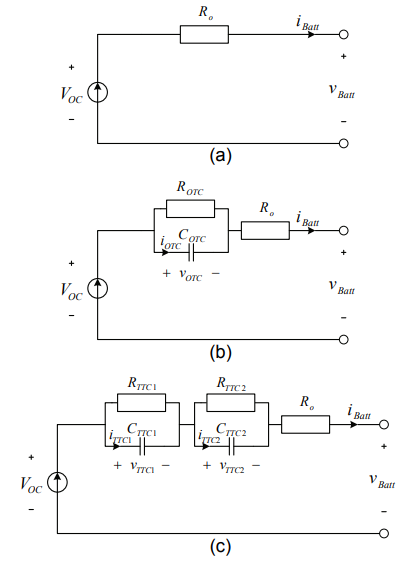
\includegraphics[width=0.5\textwidth]{Chap06/Figures/Batt_Ckt.PNG}
	\caption{Battery equivalent circuit diagrams. (a) internal resistance 
    model (IR), (b) one-time constant model (OTC), (c) two time 
    constants model (TTC) \cite{UKEMPT_AHMAD2012},\cite{UKEMPT_AHMAD2012} }
	\label{fig:Battery_Equivalent_circuit}
\end{figure}

\subsection{Nomenclature of Battery Model}
\begin{enumerate}
	\item \textbf{\textit{\underline{Open Circuit Voltage(OCV) }:}} OCV is measured at the battery's open circuit terminal voltage at various SOC points when the battery is in equilibrium. A polynomial equation is used to determine the nonlinear relationship between SOC and OCV. The figure \ref{fig:Battery_OCV_Vs_Soc} displays an OCV subsystem. Because SOC directly affects OCV's value, the OCV subsystem includes a SOC computation component. The value of OCV controls the regulated voltage source. The voltage curve of the pulse discharge test (PDT) during relaxation can be used to determine the OCV value\cite{Batt_Modeling_Kharisma}.
	\item \textbf{\textit{\underline{Internal Resistanse (R0) }:}} Internal resistance results in a voltage drop in the equivalent circuit. Fig. \ref{fig:Battery_Equivalent_circuit}(a), displays the value of the subsystem R0
	as a function of the input current and SOC. A switchable resistor
	utilized to transmit a resistor's internal value's physical signal.
	From this, one can calculate the amount of internal resistance.
	Instantaneous voltage following the release of the current pulse. 
	The optimal 2-D lookup table is selected using
	the interpolation-extrapolation lookup method for R0's value\cite{Batt_Modeling_Kharisma}.
	\item \textbf{\textit{\underline{Transient Response (R1,C1,R2,C2) }:}} Transient response in this model is represented by RC.
	The transient model is again classified based on the time constant for instance $R1\times C1 = \tau 1$ is a one-time constant model and $R2\times C2 = \tau 2$  is the two-time constant model; Figure \ref{fig:Battery_Equivalent_circuit}(b) and Figure \ref{fig:Battery_Equivalent_circuit}(c). Increasing the Time constant model will serve as a realistic model battery\cite{Batt_Modeling_Kharisma}.
\end{enumerate}

\begin{figure}[h]
	\centering
	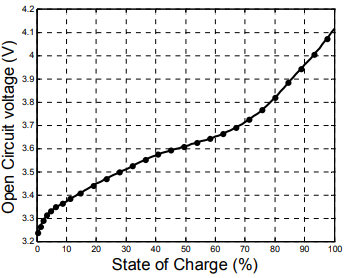
\includegraphics[width=0.5\textwidth]{Chap06/Figures/Batt_OCV_SOC.PNG}
	\caption{Battery OCV Vs Soc for SLPB120216216 Cell \cite{UKEMPT_AHMAD2012}}
	\label{fig:Battery_OCV_Vs_Soc}
\end{figure}

\subsection{IR Model :}
the IR model as shown in Figure r\ref{fig:Battery_Equivalent_circuit} (a), and 
described by Equation \ref{eq:Batt_IR_equation} implements an ideal voltage 
source VOC that represents the open-circuit voltage (OCV) 
of the battery, and an ohmic resistance to describe 
the internal resistance \cite{UKEMPT_AHMAD2012}. Both resistance and open-circuit 
voltage VOC are functions of SOC, state of health (SOH) 
and temperature. $I_{Batt}$ is the battery output current with a 
positive value when discharging, and a negative value when 
charging, $V_{Batt}$ is the battery terminal voltage\cite{UKEMPT_AHMAD2012}.

\begin{equation}\label{eq:Batt_IR_equation}
    V_{Batt} = V{OC} - R_{0}\times I_{Batt}
\end{equation}
Given that the transient is not represented by the IR model
Lithium-ion cell behavior is not suited for the
precise SOC calculation for any dynamical operation
(variable load).

\subsection{One-Time Constant Model }
A parallel RC is added by the OTC model.
Network connected in series to the IR's internal resistance R0
model to approximate the lithium-ion battery's dynamic behavior.
As shown in Figure \ref{fig:Battery_Equivalent_circuit} (b), it mainly 
consists of three parts including the voltage source $V_{OC}$, the 
ohmic resistance R0, and $R_{OTC}$,$C_{OTC}$ to describe the battery 
transient response during charging or discharging. $\textit{V}_{OTC}$ is 
the voltage across $C_{OTC}$; $i_{OTC}$ is the current that flows in 
$C_{OTC}$ \cite{UKEMPT_AHMAD2012} $\dot{\textit{V}_{OTC}}$ is the iterative voltage of OTC model. The electric behavior of the OTC model can be 
expressed by Equations \ref{eq:OTC_Voltage } and \ref{eq:OTC_Batt_Voltage } \cite{UKEMPT_AHMAD2012} in continuous time \cite{UniPadua_Giacomo}: 

\begin{equation}\label{eq:OTC_Voltage }
    \dot{ V_{OTC}} = \frac{-1}{R_{OTC}\times C_{OTC}} V_{OTC} + \frac{1}{C_{OTC}} i_{Batt}
\end{equation}
\begin{equation}\label{eq:OTC_Batt_Voltage }
    V_{Batt} = V_{OC} -  \frac{1}{C_{OTC}} V_{OTC} - R_{0}\times i_{Batt}
\end{equation}
The equation\ref{eq:Discrete_OTC_Voltage } and \ref{eq:Discrete_OTC_Batt_Voltage } (where: $T_S$ sampling period, $T_s$ and $\tau_{OTC}$  time constant. ) represents the discrete time voltages of the one-time constant model, They are very much helpful for the advanced algorithms to calculate the SoC such as Kalman, Extended Kalman etc.
\begin{equation}\label{eq:Discrete_OTC_Voltage }
    V_{OTC,k+1} = e^{\frac{-T_{s}}{\tau_{otc}}} V_{OTC,k} + R_{OTC}\left(1- e^{\frac{-T_{s}}{\tau_{otc}}}\right) i_{Batt,k}
\end{equation}
\begin{equation}\label{eq:Discrete_eOTC_Batt_Voltage }
    V_{Batt,k} = V_{OC}(SOC_{k}) -  V_{OTC,k} - R_{0}\times i_{Batt}
\end{equation}

\subsection{Two-Time Constant Model }
Model TTC, It has been discovered that the battery exhibits a significant variation between the short- and long-term transient behavior based on observation of the battery output voltage when the battery output current is zero (no load). Therefore, the OTC model cannot adequately describe the dynamic properties.
\\
An additional RC network is connected in series with the OTC circuit to create the TTC circuit model, which increases the flexibility of the OTC model.
As shown in Figure \ref{fig:Battery_Equivalent_circuit} (c), the TTC circuit is 
composed of four parts: voltage source $V_{OC}$, ohmic 
resistance $R_{O}$, $T_{TTC1}$ and $C_{TTC1}$ to describe the short term 
characteristics, $R_{TTC2}$ and $C_{TTC2}$ to describe the long term 
characteristics. $v_{TTC1}$ and $v_{TTC2}$ are the voltages across $C_{TTC1}$
and $C_{TTC2}$ respectively\cite{UKEMPT_AHMAD2012}. $i_{TTC1}$ and $i_{TTC2}$ are the outflows 
currents of $C_{TTC1}$ and $C_{TTC2}$ respectively \cite{UniPadua_Giacomo}. 

Equations \ref{eq:TTC_Voltage1 }, \ref{eq:TTC_Voltage2 }, and \ref{eq:TTC_Batt_Voltage } can be used to represent the electrical behavior of the TTC circuit in continuous time.
\begin{equation}\label{eq:TTC_Voltage1 }
    V_{TTC1} = \frac{-1}{R_{TTC1}\times C_{TTC1}} V_{TTC1} + \frac{1}{C_{TTC1}} i_{Batt}
\end{equation}
\begin{equation}\label{eq:TTC_Voltage2 }
    V_{TTC2} = \frac{-1}{R_{TTC2}\times C_{TTC2}} V_{TTC2} + \frac{1}{C_{TTC2}} i_{Batt}
\end{equation}
\begin{equation}\label{eq:TTC_Batt_Voltage }
    V_{Batt} = V_{OC} -  V_{TTC1} - V_{TTC2} - R_{0}\times i_{Batt}
\end{equation}

The TTC model equations' description in discrete time is given by Equations \ref{eq:Discrete_TTC_Voltage1 }, \ref{eq:Discrete_TTC_Voltage2 } and \ref{eq:Discrete_TTC_Batt_Voltage }:
\begin{equation}\label{eq:Discrete_TTC_Voltage1 }
    V_{TTC1,k+1} = e^{\frac{-T_{s}}{\tau_{TTC1}}} V_{TTC1,k} + R_{TTC1}\left(1- e^{\frac{-T_{s}}{\tau_{TTC1}}}\right) i_{Batt,k}
\end{equation}
\begin{equation}\label{eq:Discrete_TTC_Voltage2 }
    V_{TTC2,k+1} = e^{\frac{-T_{s}}{\tau_{TTC2}}} V_{TTC2,k} + R_{TTC2}\left(1- e^{\frac{-T_{s}}{\tau_{TTC2}}}\right) i_{Batt,k}
\end{equation}
\begin{equation}\label{eq:Discrete_TTC_Batt_Voltage }
    V_{Batt,k} = V_{OC}(SOC_{k}) -  V_{TTC1,k}-  V_{TTC2,k} - R_{0}\times i_{Batt}
\end{equation}


\subsection{Estimation of the Model Parameters}\label{sec:Batt_model_parameters_estimation}
This section demonstrates the process for estimating model parameters based on battery readings. First, the effects of temperature and aging are disregarded. At a constant temperature of 25°C, the experimental parameter identification of the battery was carried out using recently manufactured, unused cells. Figure \ref{fig:Battery_Current_Pulse} shows the typical Battery Charging and discharging behavior for the large current pulse. A continuation of this work will take into account the effects of temperature and aging.
\subsubsection{Charging and Discharging :}
Figure \ref{fig:Battery_Current_Pulse} displays the voltage and current output characteristic curves of a battery during charging and discharging. 
Following is a description of the various curve subintervals:

\begin{itemize}
	\item \textbf{Subinterval $S_0 (t < t_0 )$ :} In this subinterval the battery 
	the output current can be assumed to zero over a sufficient 
	time, though the output voltage can reach the open circuit 
	voltage value $V_{OC}(SOC_0)$, and while the output current is 
	zero the SOC value is constant \cite{UKEMPT_AHMAD2012},\cite{UniPadua_Giacomo}.
	\item \textbf{Subinterval $S_1 (t_0 \leq t \leq  t_1 )$ :}  In this subinterval the battery 
	is discharged with a constant current $I_{discharge} > 0$, first  
	a steep decrease in the battery output voltage can be seen 
	due to the internal resistance R0, and then it continues to 
	decrease exponentially controlled by the OCV (as the SOC 
	is decreasing)\cite{UKEMPT_AHMAD2012}. 
	\item \textbf{Subinterval $S_2 (t_1 \leq t \leq  t_2 )$ :} In this subinterval the battery 
	output current $i_{Batt} = 0$, so the battery output voltage at first 
	will have a steep increase due to $R_0$, and then it shows an 
	exponential increase until it reaches $V_{OC}(SOC_1)$. 
	\item \textbf{Subinterval $S_3 (t_2 \leq t \leq  t_3 )$ :} In this subinterval the battery 
	is charged with a constant current $I_{charge} < 0$; at first a steep 
	increase in the battery output voltage can be seen due to 
	internal resistance $R_0$, and then it continues to increase 
	exponentially controlled by the OCV (as the SOC is 
	increasing)\cite{UKEMPT_AHMAD2012}.
	\item \textbf{Subinterval $S_4 (t_3 \leq t \leq  t_4 )$ :} In this time subinterval the battery 
	output current $i_{Batt} = 0$, so the battery output voltage at first 
	will have a steep decrease due to $R_0$, and then it has an 
	exponential decrease until it reaches $V_{OC}(SOC_2)$ \cite{UKEMPT_AHMAD2012}. 
\end{itemize}

\begin{figure}[h]
	\centering
	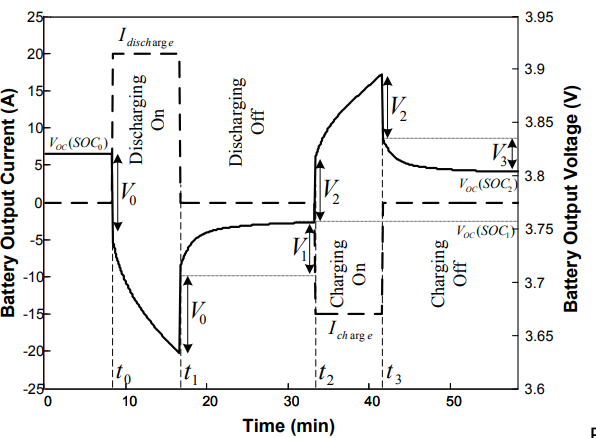
\includegraphics[width=0.5\textwidth]{Chap06/Figures/Batt_Pulsed_current_char.PNG}
	\caption{Characteristic waveforms for battery output voltage and current during charging and discharging of lithium-ion cells.}
	\label{fig:Battery_Current_Pulse}
\end{figure}

\paragraph{Ohmic Resistance :} 
The voltage drop across R0 at the 
first time instant when charging ($V_2$) respectively 
discharging ($V_0$) can be taken to calculate $R_0$ \cite{Internal_Resistance_LIPO_Batt_Gogoana}, according 
to Equation \ref{eq:Batt_Ohmic_Resistance}: 

\begin{equation}\label{eq:Batt_Ohmic_Resistance}
	R_0 =\begin{cases}
	  \frac{V_0}{I_{discharge}}, & \text{: for discharge}.\\
	  \frac{- V_2}{I_{discharge}}, & \text{: for charge}.\\
	\end{cases}
\end{equation}

\paragraph{Estimation of the OTC Model Parameters :} 
in this step 
battery output voltage measurements during the 
subintervals S2 and S4 are used, as in these subintervals 
OCV is constant\cite{Internal_Resistance_LIPO_Batt_Gogoana}, and the battery output voltage is just 
driven by the dynamic characteristics of the battery. The 
output voltage $v_{Batt}$ during S2 and S4 can be calculated 
according to the OTC model by setting $i_{Batt}$ to zero in 
Equations \ref{eq:OTC_Voltage } and \ref{eq:OTC_Batt_Voltage }, then solving the differential equation as 
shown in Equation \ref{eq:Batt_OTC_Diff_Eq_Sol} \cite {UKEMPT_AHMAD2012}:

\begin{equation}\label{eq:Batt_OTC_Diff_Eq_Sol}
	\begin{cases}
	  S_2 : V_{Batt}(t) = V_{OC}(SOC_1) - v_{OTC}(t1) e^{\frac{-t}{\tau_{OTC}}} , & \text{:where,} \tau_{OTC} = R_{OTC}\times C_{OTC}.\\
	  S_4 : V_{Batt}(t) = V_{OC}(SOC_2) - v_{OTC}(t3) e^{\frac{-t}{\tau_{OTC}}}\\
	\end{cases}
\end{equation}

Estimating the values is necessary for the identification of OTC model parameters $V_{OC}(SOC_1),V_{OC}(SOC_2),v_{OTC}(t1),v_{OTC}(t3), \tau_{OTC}$  
in Equations \ref{eq:Batt_OTC_Diff_Eq_Sol}. A nonlinear least squares approach is used (also known as nonlinear data fitting) to find the values that best suit the relationship between the measurements and the nonlinear function, in this case, an exponential function, to estimate these parameters
$f(t) = A + Be^{-\alpha t}$ . \\

The vector of coefficients A, B, and $\alpha$ is the result of the nonlinear least squares algorithm. Through Equations \ref{eq:Batt_OTC_Least_Square_solution} to \ref{eq:Batt_OTC_C_OTC}, these coefficients will be used to calculate the OTC model parameters:

\begin{equation}\label{eq:Batt_OTC_Least_Square_solution}
	\begin{cases}
	  S_2 : V_{OC}(SOC_1) = A, v_{OTC}(t1) = B, & \text{:where,} \tau_{OTC} = \frac{1}{\alpha}.\\
	  S_4 : V_{OC}(SOC_2) = A, v_{OTC}(t2) = B,\\
	\end{cases}
\end{equation}

\begin{equation}\label{eq:Batt_OTC_T_charge_discharge}
	\begin{cases}
		T_{Charge} = t1 - t0\\
		T_{Discharge} = t3 - t2 \\
	\end{cases}
\end{equation}

\begin{equation}\label{eq:Batt_OTC_R_OTC}
	\begin{cases}
	  S_2 : R_{OTC} = \frac{v_{OTC}(t1)}{ \left( 1 - e^{\frac{- T_{Discharge} }{\tau_{OTC} }}\right) I_{Discharge}} \\
	  S_4 : R_{OTC} = \frac{v_{OTC}(t3)}{ \left( 1 - e^{\frac{- T_{Charge} }{\tau_{OTC} }}\right) I_{Charge}} \\
	\end{cases}
\end{equation}

\begin{equation}\label{eq:Batt_OTC_C_OTC}
	C_{OTC} = \frac{\tau_{OTC}}{R_{OTC}}
\end{equation}

\paragraph{Estimation of the TTC Model Parameters :} 

By considering the two RC networks in place of the OTC model's single RC network, the TTC model parameters can be calculated in the same manner as for the OTC model. Equations \ref{eq:Batt_TTC_Diff_Eq_Sol} can be used to define the output voltage of the TTC model for the subintervals S2 and S4. The experiments carried out on the LIPO Battery and the typical parameters of the Battery are shown in table 4.1.

\begin{equation}\label{eq:Batt_TTC_Diff_Eq_Sol}
	\begin{cases}
	  S_2 : V_{Batt}(t) = V_{OC}(SOC_1) - v_{TTC1}(t1) e^{\frac{-t}{\tau_{TTC1}}} - v_{TTC2}(t1) e^{\frac{-t}{\tau_{TTC2}}},&\tau_{TTC1} = R_{TTC1}\times C_{TTC1}.\\
	  S_4 : V_{Batt}(t) = V_{OC}(SOC_2) - v_{TTC1}(t3) e^{\frac{-t}{\tau_{TTC1}}} - v_{TTC2}(t3) e^{\frac{-t}{\tau_{TTC2}}},&\tau_{TTC2} = R_{TTC2}\times C_{TTC2}. \\
	\end{cases}
\end{equation}


\begin{table}[ht]\label{tb:SLPB120216216_Cell_Data }
	\begin{center}
		\begin{tabular}{|c|c|c|}
			\hline
			\multicolumn{2}{|c|}{{Typical Capacity }} & 53 Ah\\
			\hline
			\multicolumn{2}{|c|}{{Nominal Voltage}} & 3.7\\
			\hline
			\multicolumn{1}{|c|}{\multirow{2}{*}{Charge Condition}}& Max. Current & 53A\\ 
			\multicolumn{1}{|c|}{}& Voltage & 4.2V $\frac{+}{-}$ 0.03V\\
			\hline
			\multicolumn{1}{|c|}{\multirow{2}{*}{Discharge Condition}}& Max. Current & 159A\\
			\multicolumn{1}{|c|}{}& Peak Current & 290A\\
			\multicolumn{1}{|c|}{}& Cut-off Voltage & 3.0V\\
			\hline
		\end{tabular}
		\caption{SLPB120216216 Cell Data }
	\end{center}
	\label{tab:multicol}
\end{table}

Estimating the values is required for the TTC model's identification, $V_{OC}(SOC_1), V_{OC}(SOC_2), v_{TTC_1}(t1), v_{TTC_1}(t3), v_{TTC_2}(t1), 
v_{TTC_2}(t3), \tau_{TTC_1}  and  \tau_{TTC_2}$ in Equations \ref{eq:Batt_TTC_Diff_Eq_Sol}. In this 
case an exponential function with two-time constants $f(t)=A+Be^{-\alpha t}+Ce^{- \beta t}$ is used.
\\
The vector of coefficients A, B, C,$\alpha, and \beta$ is the result of the nonlinear least squares algorithm. Through Equations \ref{eq:Batt_OTC_Least_Square_solution} to \ref{eq:Batt_TTC_C_TTC}, these coefficients will be utilized to calculate all the TTC model's parameters. 

\begin{equation}
	\begin{cases}
	  S_2 : V_{OC}(SOC_1) = A 
	  S_4 : V_{OC}(SOC_2) = A
	\end{cases}
\end{equation}

\begin{equation}\label{eq:Batt_OTC_Least_Square_solution}
	\begin{cases}
	  S_2 :  v_{TTC1}(t1) = B, v_{TTC2}(t1) = C ,& \text{:} \tau_{TTC1} = \frac{1}{\alpha}.\\
	  S_4 :  v_{TTC1}(t3) = B, v_{TTC2}(t3) = C ,& \text{:} \tau_{TTC2} = \frac{1}{\beta}.\\
	\end{cases}
\end{equation}

\begin{equation}\label{eq:Batt_TTC_R_TTC1}
	\begin{cases}
	  S_2 : R_{TTC1} = \frac{v_{TTC1}(t1)}{ \left( 1 - e^{\frac{- T_{Discharge} }{\tau_{TTC1} }}\right) I_{Discharge}} \\
	  S_4 : R_{TTC1} = \frac{v_{TTC1}(t3)}{ \left( 1 - e^{\frac{- T_{Charge} }{\tau_{TTC1} }}\right) I_{Charge}} \\
	\end{cases}
\end{equation}

\begin{equation}\label{eq:Batt_TTC_R_TTC2}
	\begin{cases}
	  S_2 : R_{TTC2} = \frac{v_{TTC2}(t1)}{ \left( 1 - e^{\frac{- T_{Discharge} }{\tau_{TTC2} }}\right) I_{Discharge}} \\
	  S_4 : R_{TTC2} = \frac{v_{TTC2}(t3)}{ \left( 1 - e^{\frac{- T_{Charge} }{\tau_{TTC2} }}\right) I_{Charge}} \\
	\end{cases}
\end{equation}

\begin{equation}\label{eq:Batt_TTC_C_TTC}
	\begin{cases}
		C_{TTC1} = \frac{\tau_{TTC1}}{R_{TTC1}} \\
		C_{TTC2} = \frac{\tau_{TTC2}}{R_{TTC2}} \\
	\end{cases}
\end{equation}

\subsection{Experimental and Computational Results of SLPB120216216}
Cells made of lithium polymer by the producer Kokam were employed for the modeling and experimental experiments.
Table 4.1 shows several significant cell data. A battery test bench was established to determine the model parameters. Using short and long interruptions, a rectangular-shaped current signal must be applied to the battery on this test bench. It is also necessary to measure the voltage of the battery output. While the OTC and TTC model parameters must be determined during extended pauses, the battery's ohmic resistance R0 can be measured during small interruptions of the current signal.

\begin{figure}[h]
	\centering
	\subfigure[Ohmic Resistance $R_0 = f(SOC) @ Discharging $]{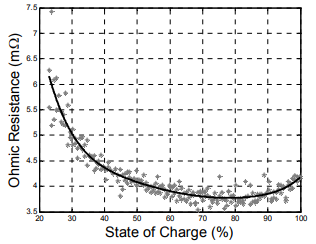
\includegraphics[scale=.8]{Chap06/Figures/Batt_DisCh_Ohmic_Resistance.PNG}}
	\qquad
	\subfigure[Ohmic Resistance $R_0 = f(SOC) @ Chareging $]{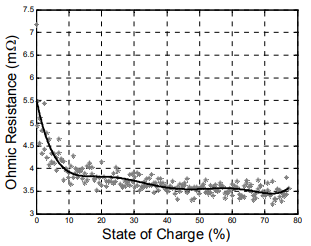
\includegraphics[scale=.8]{Chap06/Figures/Batt_Ch_Ohmic_Resistance.PNG}}
	\qquad
	\subfigure[Output Voltage of the Battery $@ Discharing$]{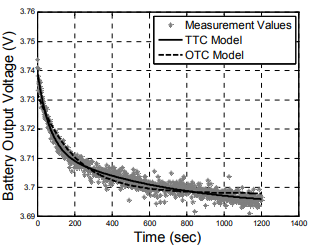
\includegraphics[scale=.8]{Chap06/Figures/Batt_DisCh_OutPut_Voltage.PNG}}
	\qquad
	\subfigure[Output Voltage of the Battery $@ Charging $]{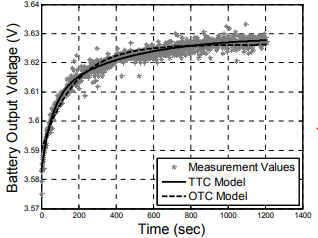
\includegraphics[scale=.8]{Chap06/Figures/Batt_Ch_OutPut_Voltage.PNG}}
	\qquad
	\subfigure[Dynamic Resistance of the Battery  $R_{OTC}/R_{TTC1}/R_{TTC_2} = f(SOC) @ Discharging $]{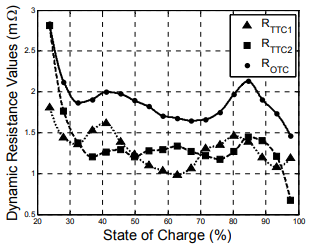
\includegraphics[scale=.8]{Chap06/Figures/Batt_DisCh_Resistance.PNG}}
	\qquad
	\subfigure[Dynamic Resistance of the Battery $R_{OTC}/R_{TTC1}/R_{TTC_2} = f(SOC) @ Charging $]{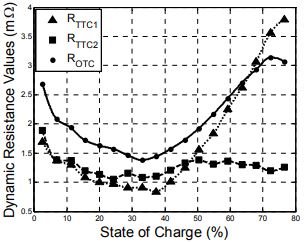
\includegraphics[scale=.8]{Chap06/Figures/Batt_Ch_Resistance.PNG}}
	\qquad
	\subfigure[Dynamic Capacitance of the Battery  $C_{OTC}/C_{TTC1}/C_{TTC_2} = f(SOC) @ Discharging $]{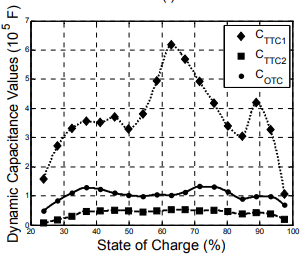
\includegraphics[scale=.8]{Chap06/Figures/Batt_DisCh_Capacitance.PNG}}
	\qquad
	\subfigure[Dynamic Capacitance of the Battery $ C_{OTC}/C_{TTC1}/C_{TTC_2} = f(SOC)  @ Charging $]{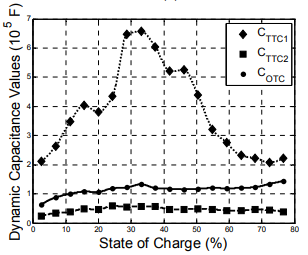
\includegraphics[scale=.8]{Chap06/Figures/Batt_Ch_Capacitance.PNG}}
	\caption{LIPo Battery SLPB120216216 Simulated Results \cite{UKEMPT_AHMAD2012} }
	\label{fig:LIPO_Batt_SLPB120216216_Results}
\end{figure}
  